\documentclass[12pt]{article}
\usepackage{caption}
\usepackage{graphicx}
\usepackage{hyperref}
\hypersetup{%
    pdfborder = {0 0 0}
}
\hypersetup{
    colorlinks,
    citecolor=blue,
    filecolor=blue,
    linkcolor=blue,
    urlcolor=blue
}
\renewcommand{\familydefault}{\sfdefault}
\renewcommand{\captionfont}{\small}

\author{Bernd Porr}
\title{Depp learning}

\begin{document}

\maketitle

\section{Lineares Neuron}

\begin{figure}[!hbt]
\begin{center}
\mbox{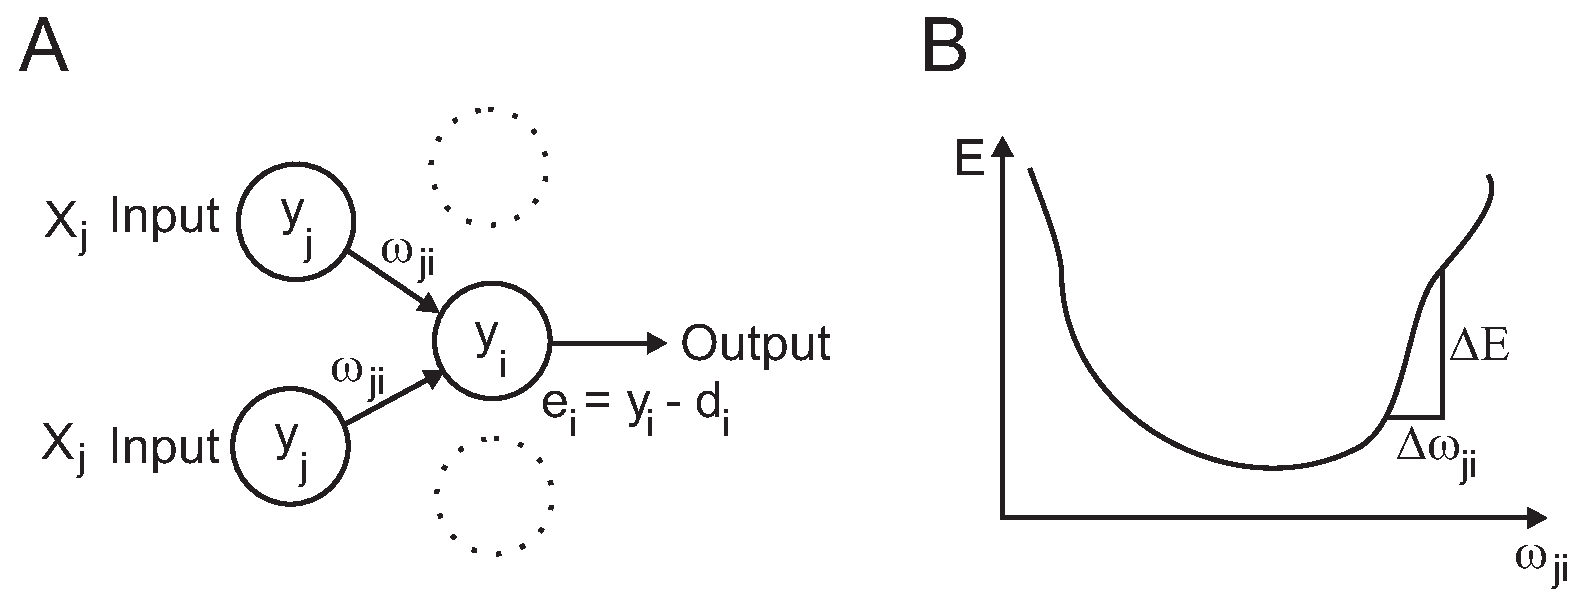
\includegraphics[width=\textwidth]{one_layer}}
\end{center}
\caption{Einfaches lineares Neuron
\label{one_layer}}
\end{figure}

Abb.~\ref{one_layer}A zeigt ein einfaches lineares Neuron in einer
einzigen Schicht. Die Aktivitaet des neurons ist $y$ und hat einen
Index fuer dessen Position in der Schicht, wobei der index $i$ hier
die Ausgangsschicht repreaesentiert. Die Eingangsaktivitaet wird mit
$\omega_{ji}$ gewichtet und dann zum Ausgangssignal $y_i$ summiert:
\begin{equation}
  y_i(n) = \sum_j y_j(n) w_{ji} \label{linear_sum}
\end{equation}

Gelernt werden soll eine bestimmte Ausgangsaktivitaet in Abhanengigkeit von einer Eingangsaktivitaet.
Das wird erreicht, indem ein Fehler $e_i$ am Ausgang jedes Neurons etabliert wird, der dann die Gewichte $w_{ji}$
schrittweise dorthin beweget, dass er im mittel Null wird:
\begin{equation}
  e_i = y_i - d_i \label{output error}
\end{equation}
wobei $d_i$ der gewuenschte Ausgangswert ist und $y_i$ der Aktuelle.
Ziel des Lernen ist es, dass das quadratische Mittel null wird:
\begin{equation}
  E = \frac{1}{2} e^2
\end{equation}

Der zentrale Trick ist nun, die Partielle Ableitung in Abhaengigkeit vom Fehler $E$ zu nehmen
und damit die Gewichte zu veraendern:
\begin{eqnarray}
  \Delta\omega_{ji} & = & - \mu \frac{\partial E}{\partial \omega_{ji}} \label{graddes} \\
  \omega_{ji} & \leftarrow & \omega_{ji} + \Delta\omega_{ji}
\end{eqnarray}
Warum macht das Sinn? In Abb.~\ref{one_layer}B ist die Abhaengigkeit von einem Gewicht
$\omega_{ji}$ gezeigt. wenn in diesem Beispiel das Gewicht etwas erhoeht wird, dann
wird der Fehler $E$ groesser also war die Erhoehung kontraproduktiv und es ist besser,
das Gewicht zu verringern. Wenn aber umgekehrt eine Erhoehung von $\omega_{ji}$ eine
Verringerung von E bewirkt, dann ist das Vorteilhaft also kann man das Gewicht erhoehen.
Iterativ wird also der Fehler verringert.

Als naechsten Schritt muss nun die Lernregel hergeleitet werden. Das geschieht, indem
mein einfach Gl.~\ref{linear_sum} in Gl.~\ref{graddes} einsetzt und die Partiellen Ableitungen
durchfuehrt:
\begin{eqnarray}
  \Delta\omega_{ji}
   & = & - \mu \frac{1}{2} \frac{\partial ( d_i(n) - y_i(n) )^2 }{\partial \omega_{ji}} \\
   & = & - \mu \frac{1}{2} \frac{\partial ( d_i(n) - \left( \sum_j y_j(n) w_{ji} \right)^2 }{\partial \omega_{ji}} \\
   & = & - \mu \frac{1}{2} \underbrace{\frac{\partial E}{\partial y_i}}_{-2e(n)} \underbrace{\frac{\partial y_i}{\partial \omega_{ji}}}_{y_j(n)} \\
  & = & \mu \underbrace{\left(d_i(n) - \sum_j y_j(n) w_{ji}\right)}_{e(n)} \cdot y_j(n) \\
  & = & \mu \cdot e_i(n) \cdot y_j(n)
\end{eqnarray}

\section{Fehlerpropagierung (linearer Fall)}
\begin{figure}[!hbt]
\begin{center}
\mbox{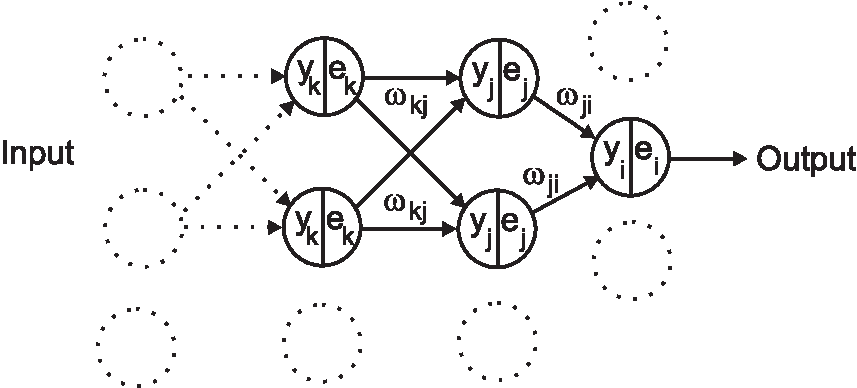
\includegraphics[width=\textwidth]{multi_layer}}
\end{center}
\caption{Mehrschichtiges Feedforward Netz
\label{multi_layer}}
\end{figure}


\end{document}
